\documentclass[a4paper]{article}

%\usepackage[document]{ragged2e}
\usepackage{fullpage} % Package to use full page
\usepackage{parskip} % Package to tweak paragraph skipping
\usepackage{tikz} % Package for drawing
\usepackage{amsmath}
\usepackage{hyperref}
\usepackage{listings}
\usepackage{float}

\title{Introduction to Intelligent Systems: Assignment 4
\\Bayes classification and Normal Distribution}
\author{Damiano Melotti (S3838706)\\Amadeus Beckmann (S3839508)\\Group 55}
\date{\today}

\begin{document}

\maketitle

\section{Assignment 1}

\begin{figure}[H]
\begin{center}
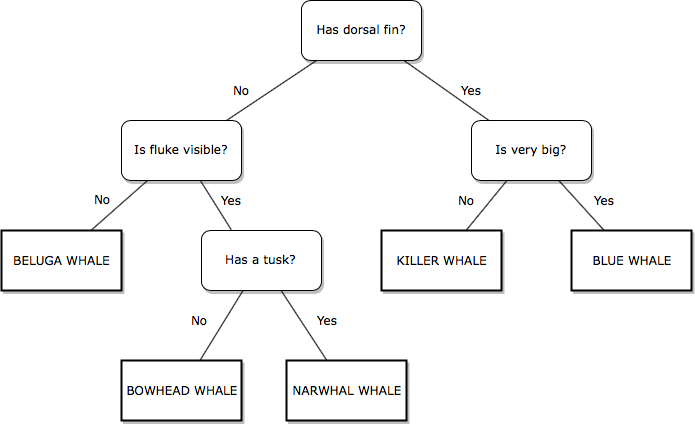
\includegraphics[width=\textwidth]{binary-decision-tree-for-whales.png}
\end{center}
\caption{Binary decision tree for whale spotters}
\label{ref:decision-tree}
\end{figure}

Figure \ref{ref:decision-tree} shows a binary decision tree that can be used to distinguish \textbf{killer whales}, \textbf{beluga whales}, \textbf{narwhals}, \textbf{bowhead whales}, and \textbf{blue whales}. Using easily identifiable characteristics, it can be determined with minimal effort which specimen is in question.

Our feature vector was: $<$size, dorsal fin, visible fluke, tusk$>$.
\begin{description}
    \item Size: [\underline{\textcolor{red}{s}}mall; \underline{\textcolor{red}{m}}edium; \underline{\textcolor{red}{l}}arge]
    \item Dorsal fin: [\underline{\textcolor{red}{pr}}esent, \underline{\textcolor{red}{n}}ot-\underline{\textcolor{red}{p}}resent]
    \item Visible fluke: [\underline{\textcolor{red}{v}}isible; \underline{\textcolor{red}{n}}ot-\underline{\textcolor{red}{v}}isible]
    \item Tusk: [\underline{\textcolor{red}{y}}es; \underline{\textcolor{red}{n}}o]
\end{description}

Considering the characteristics the marine biologist provided, we came up with the following schematization:

\textbf{Killer whale:}
\begin{enumerate}
    \item Fluke not visible when diving;
    \item Small size (6-8m);
    \item Tall and pointed dorsal fin is often clearly visible;
    \item Blows water quite often.
\end{enumerate}
Vector: $<$s,pr,nv,?$>$  

\textbf{Beluga whale:}
\begin{enumerate}
    \item No fluke when diving;
    \item No dorsal fin.
\end{enumerate}
Vector: $<$?,np,nv,?$>$

\textbf{Narwhal:}
\begin{enumerate}
    \item Very small;
    \item Long tusk;
    \item Fluke is clearly visible;
    \item No dorsal fin.
\end{enumerate}
Vector: $<$s,np,v,y$>$

\textbf{Bowhead whale:}
\begin{enumerate}
    \item Large size of 20m;
    \item Fluke is visible;
    \item No dorsal fin.
\end{enumerate}
Vector: $<$l,np,v,?$>$

\textbf{Blue whale:}
\begin{enumerate}
    \item Very large size of 30m;
    \item Impressive fluke;
    \item Small dorsal fin;
\end{enumerate}
Vector: $<$l,p,v,?$>$


Our first thought was to split the whales into two equal groups. We had to take into account that there are unknown features in some of the animals, so only two characteristics can be considered, which apply to half of the whales: the possession of a dorsal fin and the visibility of the fluke. However, we've made the possession of a \textbf{dorsal fin} the first decision.

The only two whales that have a dorsal fin are the killer whale and the blue whale. They are pretty easy to differentiate: one is 6-8m long, the other 30m. So the choice of the decision criterion for these two mammals is their \textbf{size}.

The remaining three whales, which do not have a dorsal fin are also pretty easy to distinguish, because one of them has no visible \textbf{fluke}: that is the beluga whale, which means only the narwhal and the bowhead whale remain.

Finally, it is not difficult to recognize the remaining two whales: the narwhal has a long \textbf{tusk} and the bowhead whale does not.

With this binary decision tree not only the height of the tree is minimal, but also the characteristics to determine are well recognizable.


\section{Assignment 2}

\subsection{Dendogram}

We've created the dendrogram following the given indications. To calculate the dissimilarity between the elements of our data set and generate the matrix we used the Euclidean distance. Then we created a hierarchical binary cluster tree with the default linking function offered in MATLAB, and we generated the dendrogram.

\begin{figure}[H]
\begin{center}
\includegraphics[width=\textwidth]{dendrogram.eps}
\end{center}
\caption{Dendogram of 19 stocks}
\end{figure}

\subsection{Considerations}

When looking at the dendogram, it is noticeable that the largest Euclidean distance is almost 600\% greater than the smallest. We suspected that the dendogram visualizes the similarity between the market values: a small Euclidean distance means a large correspondence between the changes of the market values and vice versa. To confirm our thesis, we have selected two examples, one with a small and one with a large Euclidean distance, and plotted their market values.

Of course, the two graphs in figure \ref{ref:aex-rds} are not equal. The still have a lot of dissimilarities. However, if you compare it with figure \ref{ref:aex-aeg}, you can see that we were right with our assumption. While AEX in figure \ref{ref:aex-aeg} has comparatively low amplitudes, the AEG graph behaves more remarkably. Almost all values are far below or above the corresponding AEX market value. The spike at $\sim110$ also intensifies this. Furthermore, while the market values in figure \ref{ref:aex-rds} lie between $-0.04$ and $0.04$, they are rather between $-0.075$ and $0.1$ in figure \ref{ref:aex-aeg}.

\begin{figure}[H]
\begin{center}
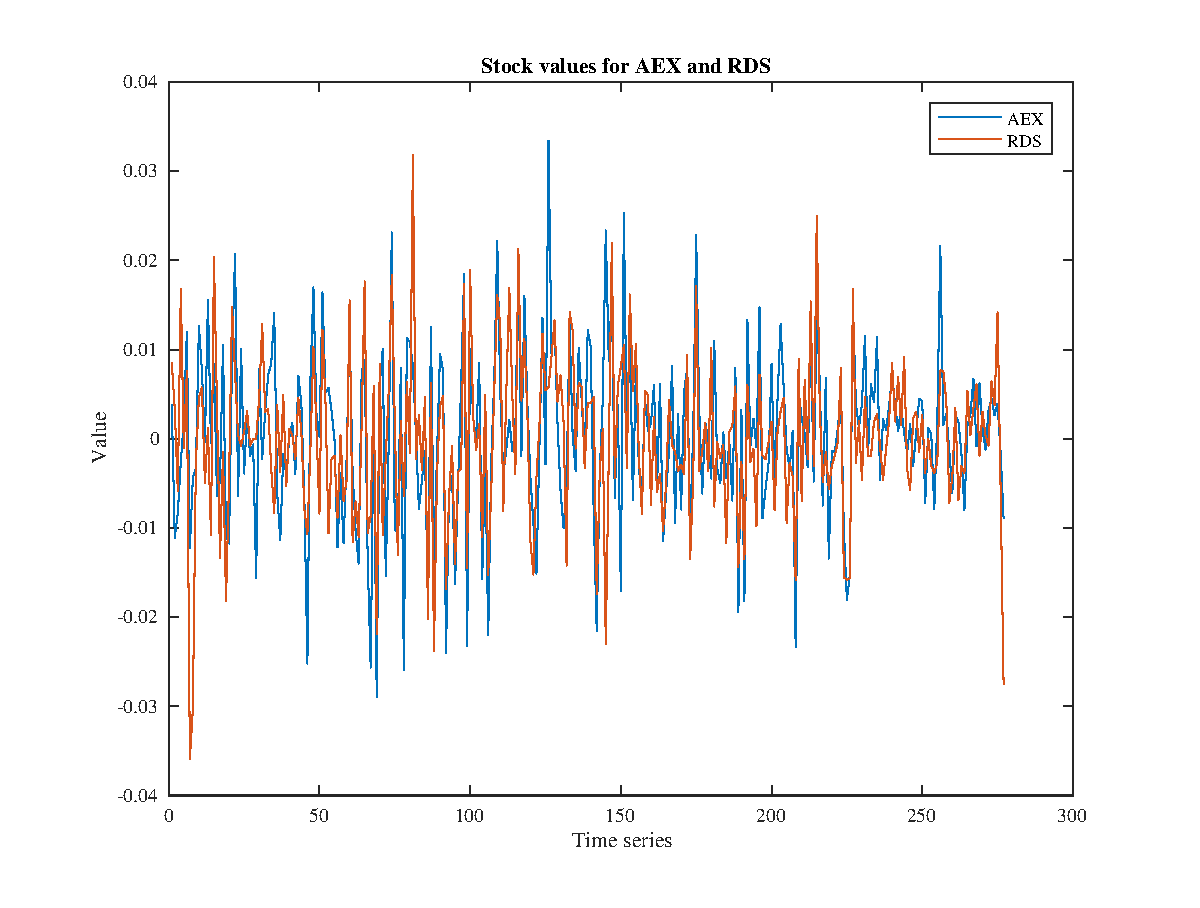
\includegraphics[width=13cm]{AEX_RDS.eps}
\label{ref:aex-rds}
\end{center}
\caption{AEX and RDS}
\end{figure}

\begin{figure}[H]
\begin{center}
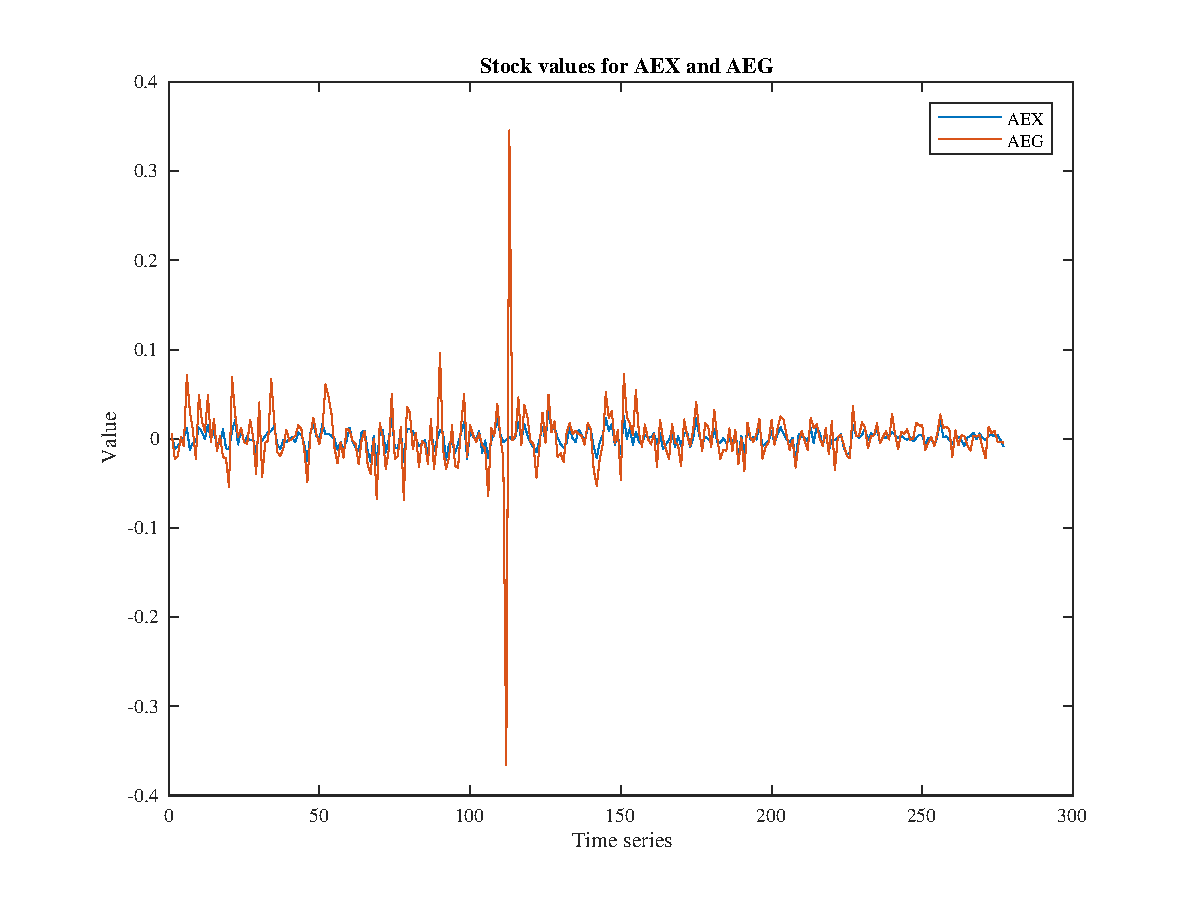
\includegraphics[width=13cm]{AEX_AEG.eps}
\label{ref:aex-aeg}
\end{center}
\caption{AEX and AEG}
\end{figure}

\subsection{Code (Dendogram)}

\begin{lstlisting}[language=Matlab]
load('lab_4_data/dataAEX.mat');
load('lab_4_data/labelsAEX.mat');

% euclidean (default) distances between the time series
distances = pdist(data);
% to visualize better the matrix
distance_matrix = squareform(distances);

% to create a hierarchical binary cluster tree
tree = linkage(distances);
% to compute the best order of leaves
leafOrder = optimalleaforder(tree, distances);

% we use introduce the labels in the plot
[H,T] = dendrogram(tree, 'Reorder', leafOrder, 'Labels', labels, 'Orientation',
'right');
title('Dendrogram of the 19 stocks');
xlabel('Euclidean distance');
ylabel('Time series');
set(gca, 'fontsize', 9.5, 'fontname', 'Times New Roman');
\end{lstlisting}

\subsection{Code (Graphs)}

\begin{lstlisting}[language=Matlab]
load('lab_4_data/dataAEX.mat');
load('lab_4_data/labelsAEX.mat');

indexAEX = find(strcmp(labels, 'AEX'), 1);
indexRDS = find(strcmp(labels, 'RDS'), 1);
indexAEG = find(strcmp(labels, 'AEG'), 1);

plot(data(indexAEX, :));
hold on;
plot(data(indexRDS, :));
legend('AEX', 'RDS');
title('Stock values for AEX and RDS');
xlabel('Time series');
ylabel('Value');
set(gca, 'fontsize', 9.5, 'fontname', 'Times New Roman');

figure(2);
plot(data(indexAEX, :));
hold on;
plot(data(indexAEG, :));
legend('AEX', 'AEG');
title('Stock values for AEX and AEG');
xlabel('Time series');
ylabel('Value');
set(gca, 'fontsize', 9.5, 'fontname', 'Times New Roman');
\end{lstlisting}

\end{document}
